\documentclass[11pt]{article}

\usepackage{pdfpages}
\usepackage{hyperref}
\usepackage{enumerate}
\usepackage{listings}
\usepackage{float}
\usepackage{amsmath}
\usepackage{changepage}
\usepackage{amssymb}
\usepackage{graphicx}%
\usepackage{subcaption}

\renewcommand*\ttdefault{lmtt}
\renewcommand*\sfdefault{lmss}
\renewcommand{\familydefault}{\sfdefault}

\begin{document}

\author{\textbf{Group 8} \\* Arian Barakat \\* Hao Chi KIANG \\* Yixuan Xu \\ Yumeng Li}

\title{Laboratory Work 3}
\maketitle

\section*{Assignment 1}

\subsection*{Matrixplot}

\begin{figure}[H]
  \centering
    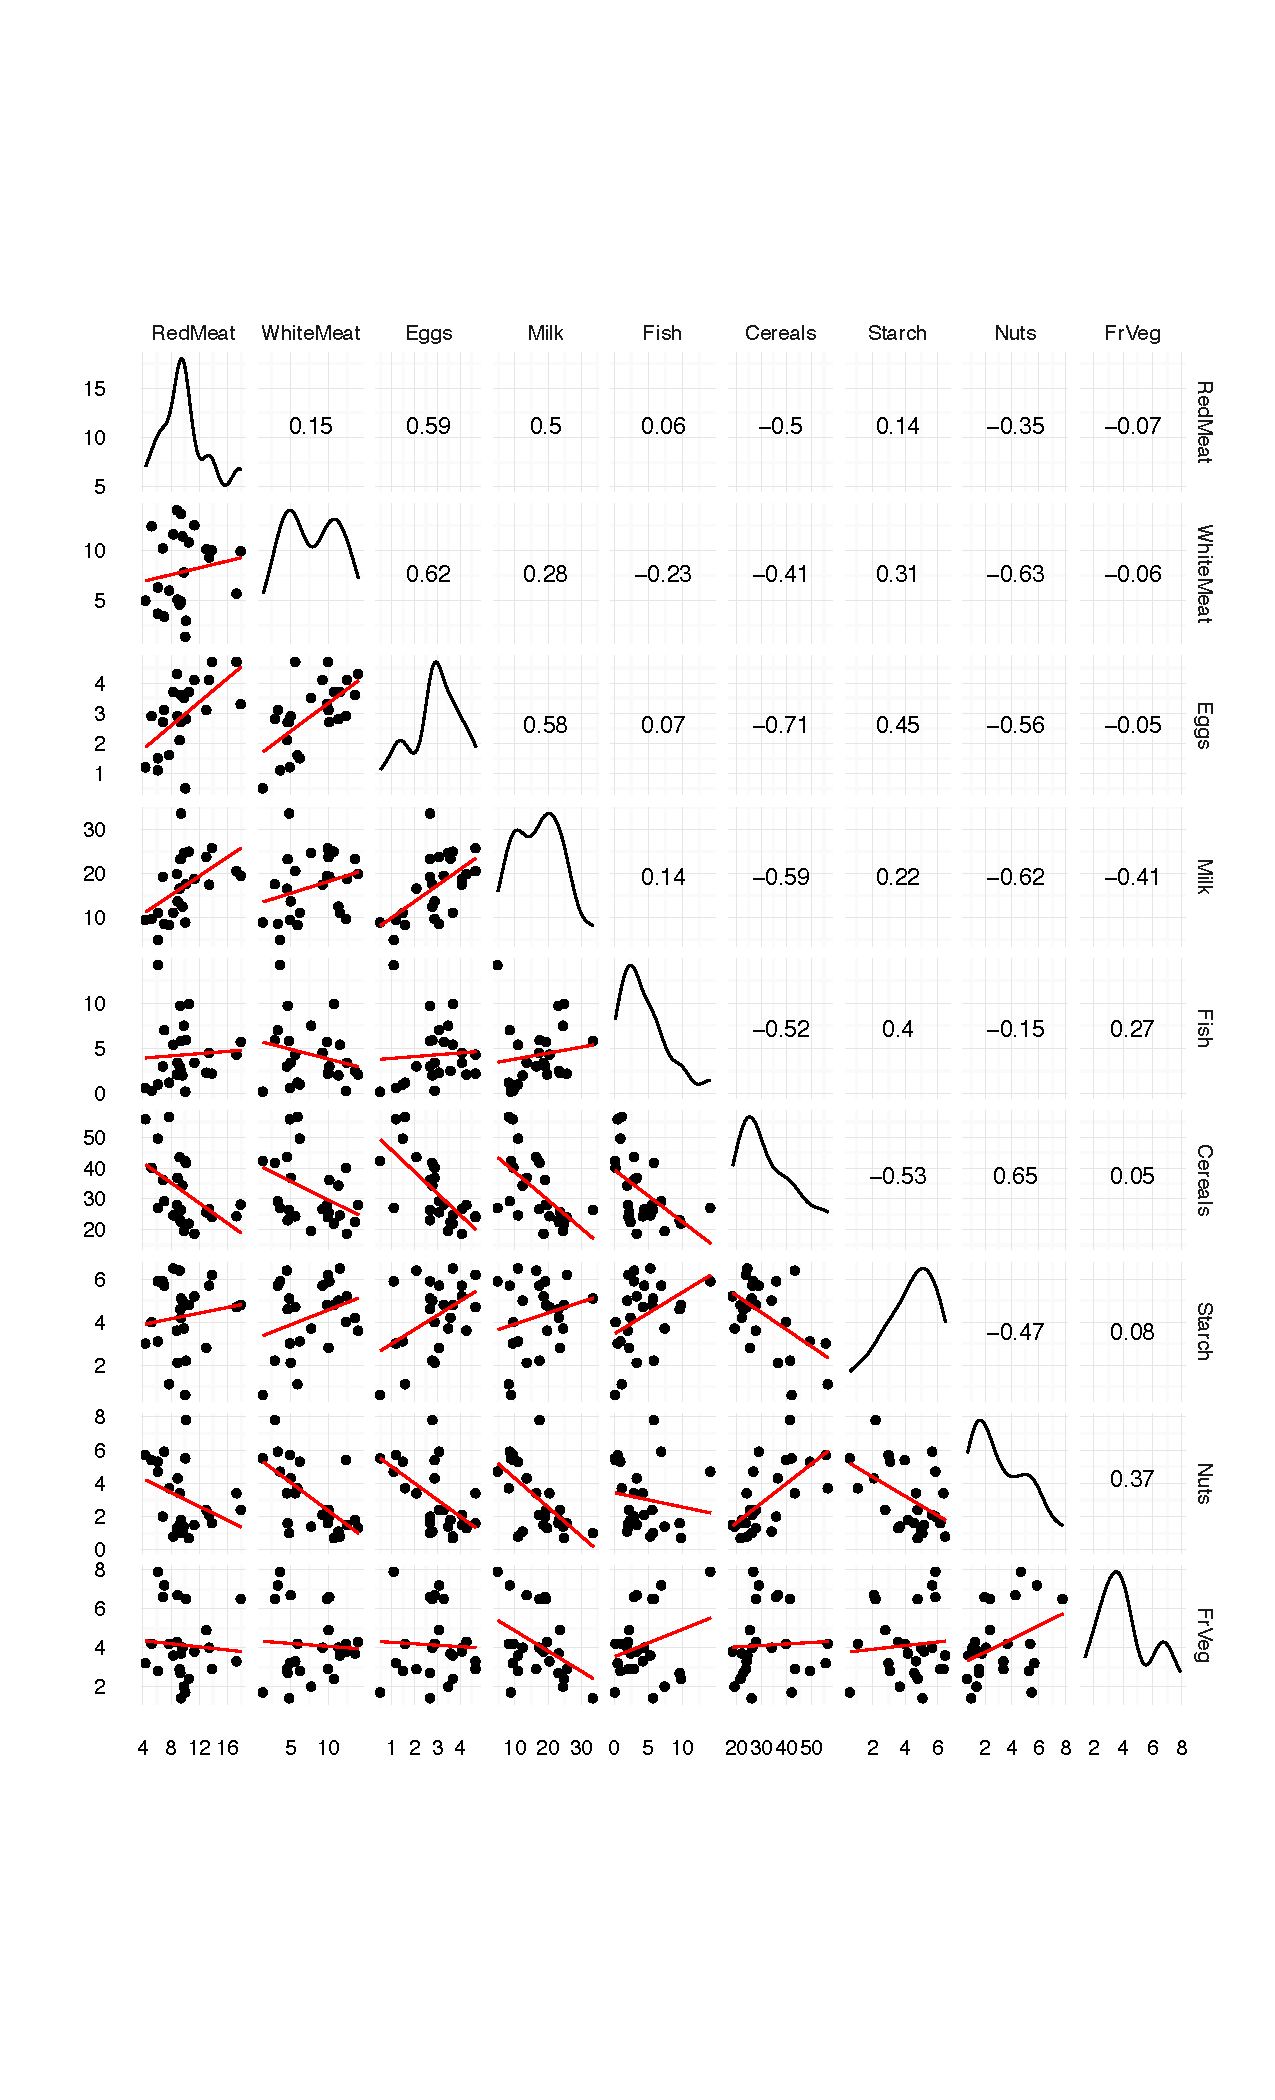
\includegraphics[height = 120mm, width = 120mm]{plot_matrix.pdf}
   \caption{Consumption of different products in different countries of Europe (quantitative measure of the amount of protein consumed), \textit{Source: protein.txt}}
   \label{fig:matrix_plot}
\end{figure}

%---- 

\subsection*{Heatmap}

\begin{figure}[H]
  \centering
    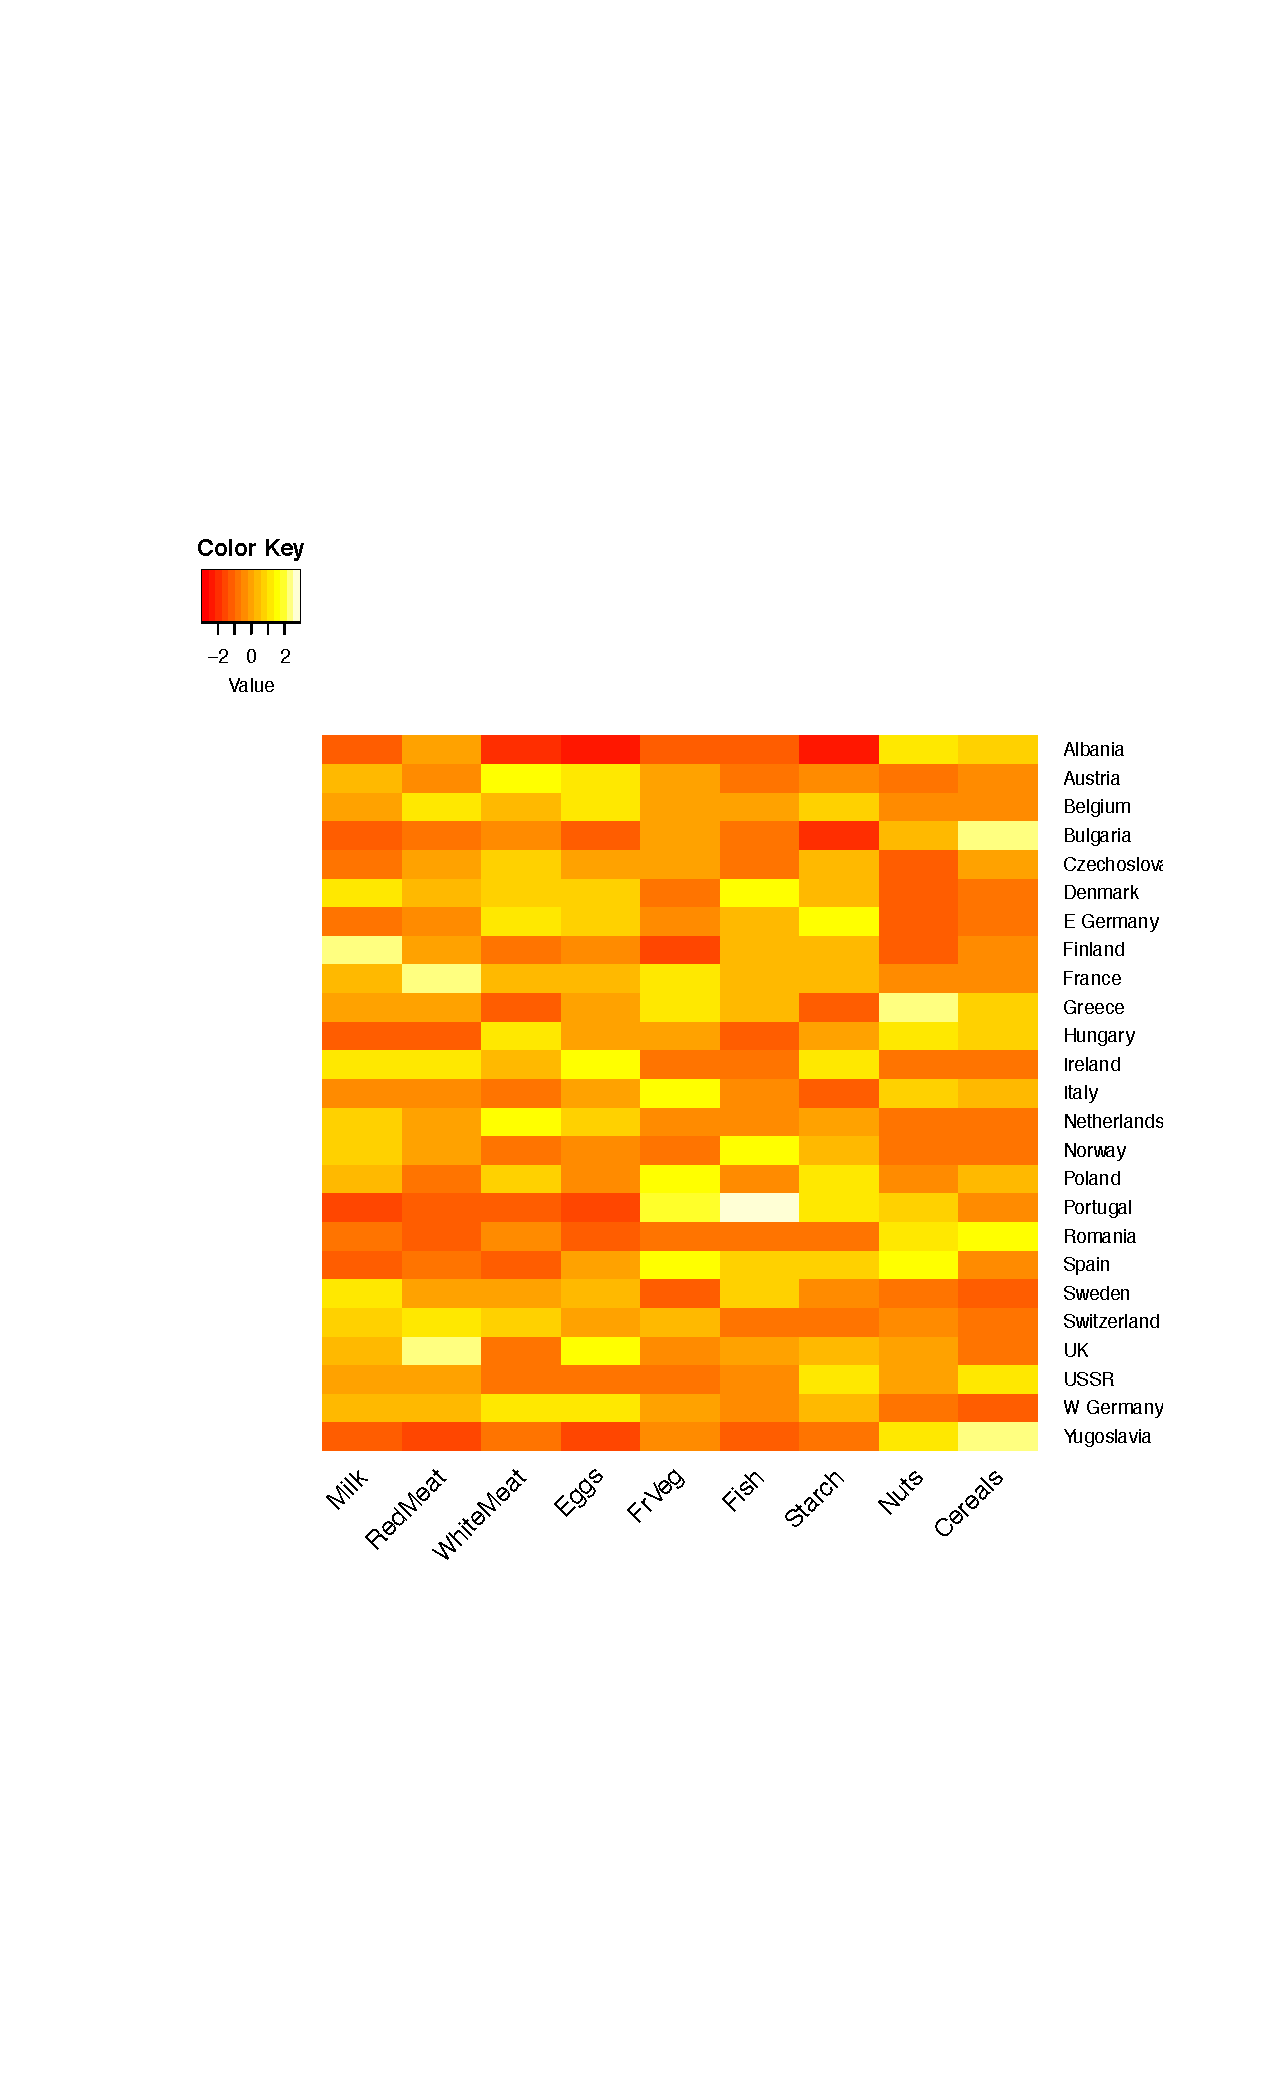
\includegraphics[scale = 0.6]{heatmap_1_2.pdf}
   \caption{Heatmap, consumption of different products in different countries of Europe (quantitative measure of the amount of protein consumed). Unpermuted and rescaled variables. \textit{Source: protein.txt} }
   \label{fig:heat_1_2}
\end{figure}

%--

\subsection*{Heatmap, Two-way hierarchical clustering}




%--

\subsection*{Heatmap, Anti-Robinson unweighted and PCA seriation}

\begin{figure}[H]
  \begin{subfigure}[h]{0.6\textwidth}
    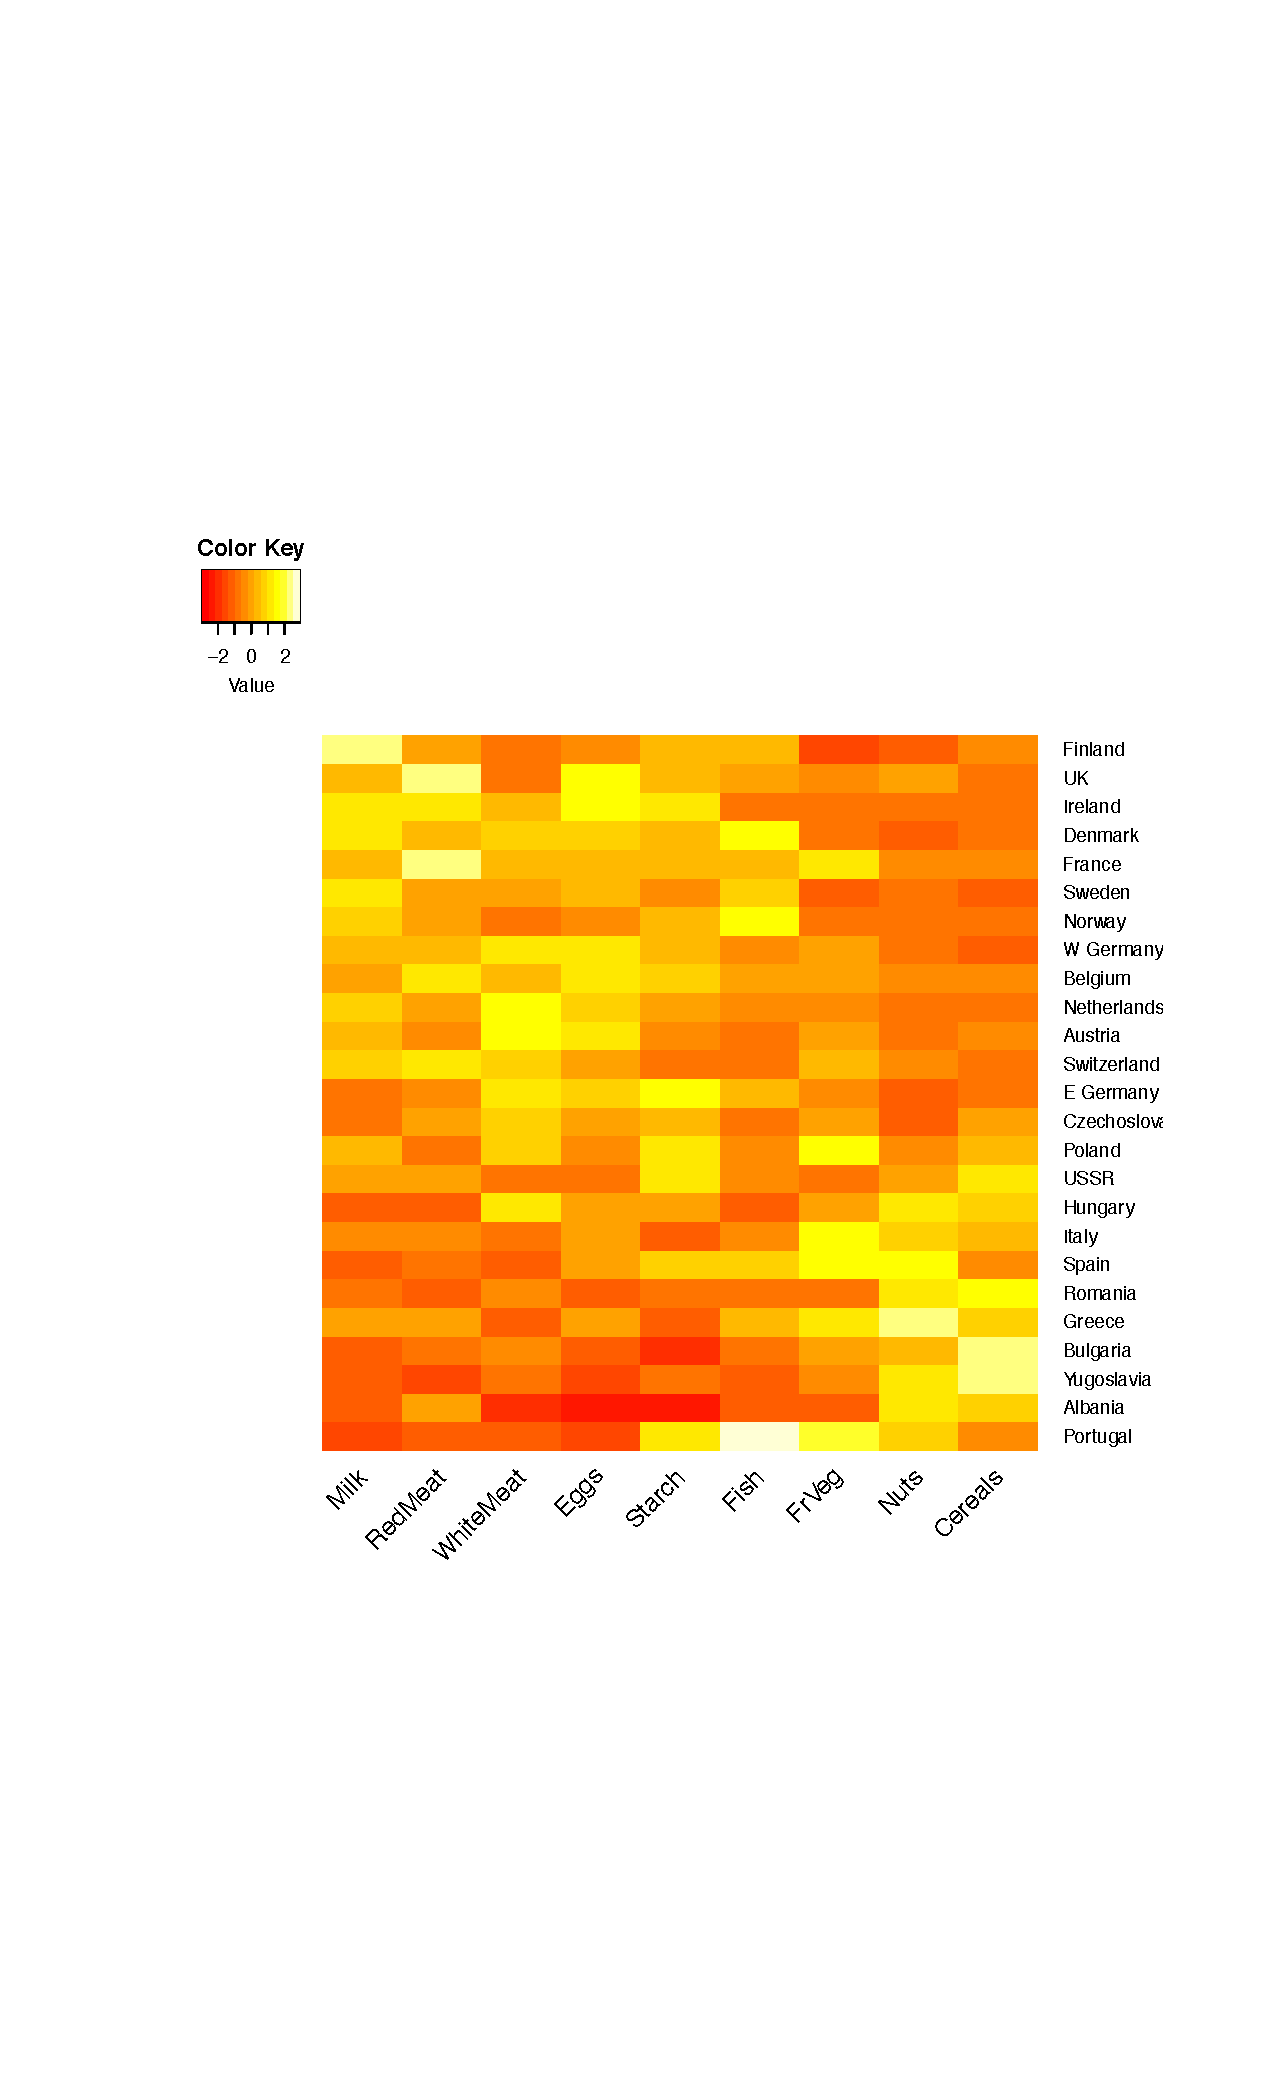
\includegraphics[width=\textwidth]{heatmap_antirobinson.pdf}
    \caption{Anti-Robinson}
    \label{fig:heat_antirob}
  \end{subfigure}
  %
  \begin{subfigure}[h]{0.6\textwidth}
    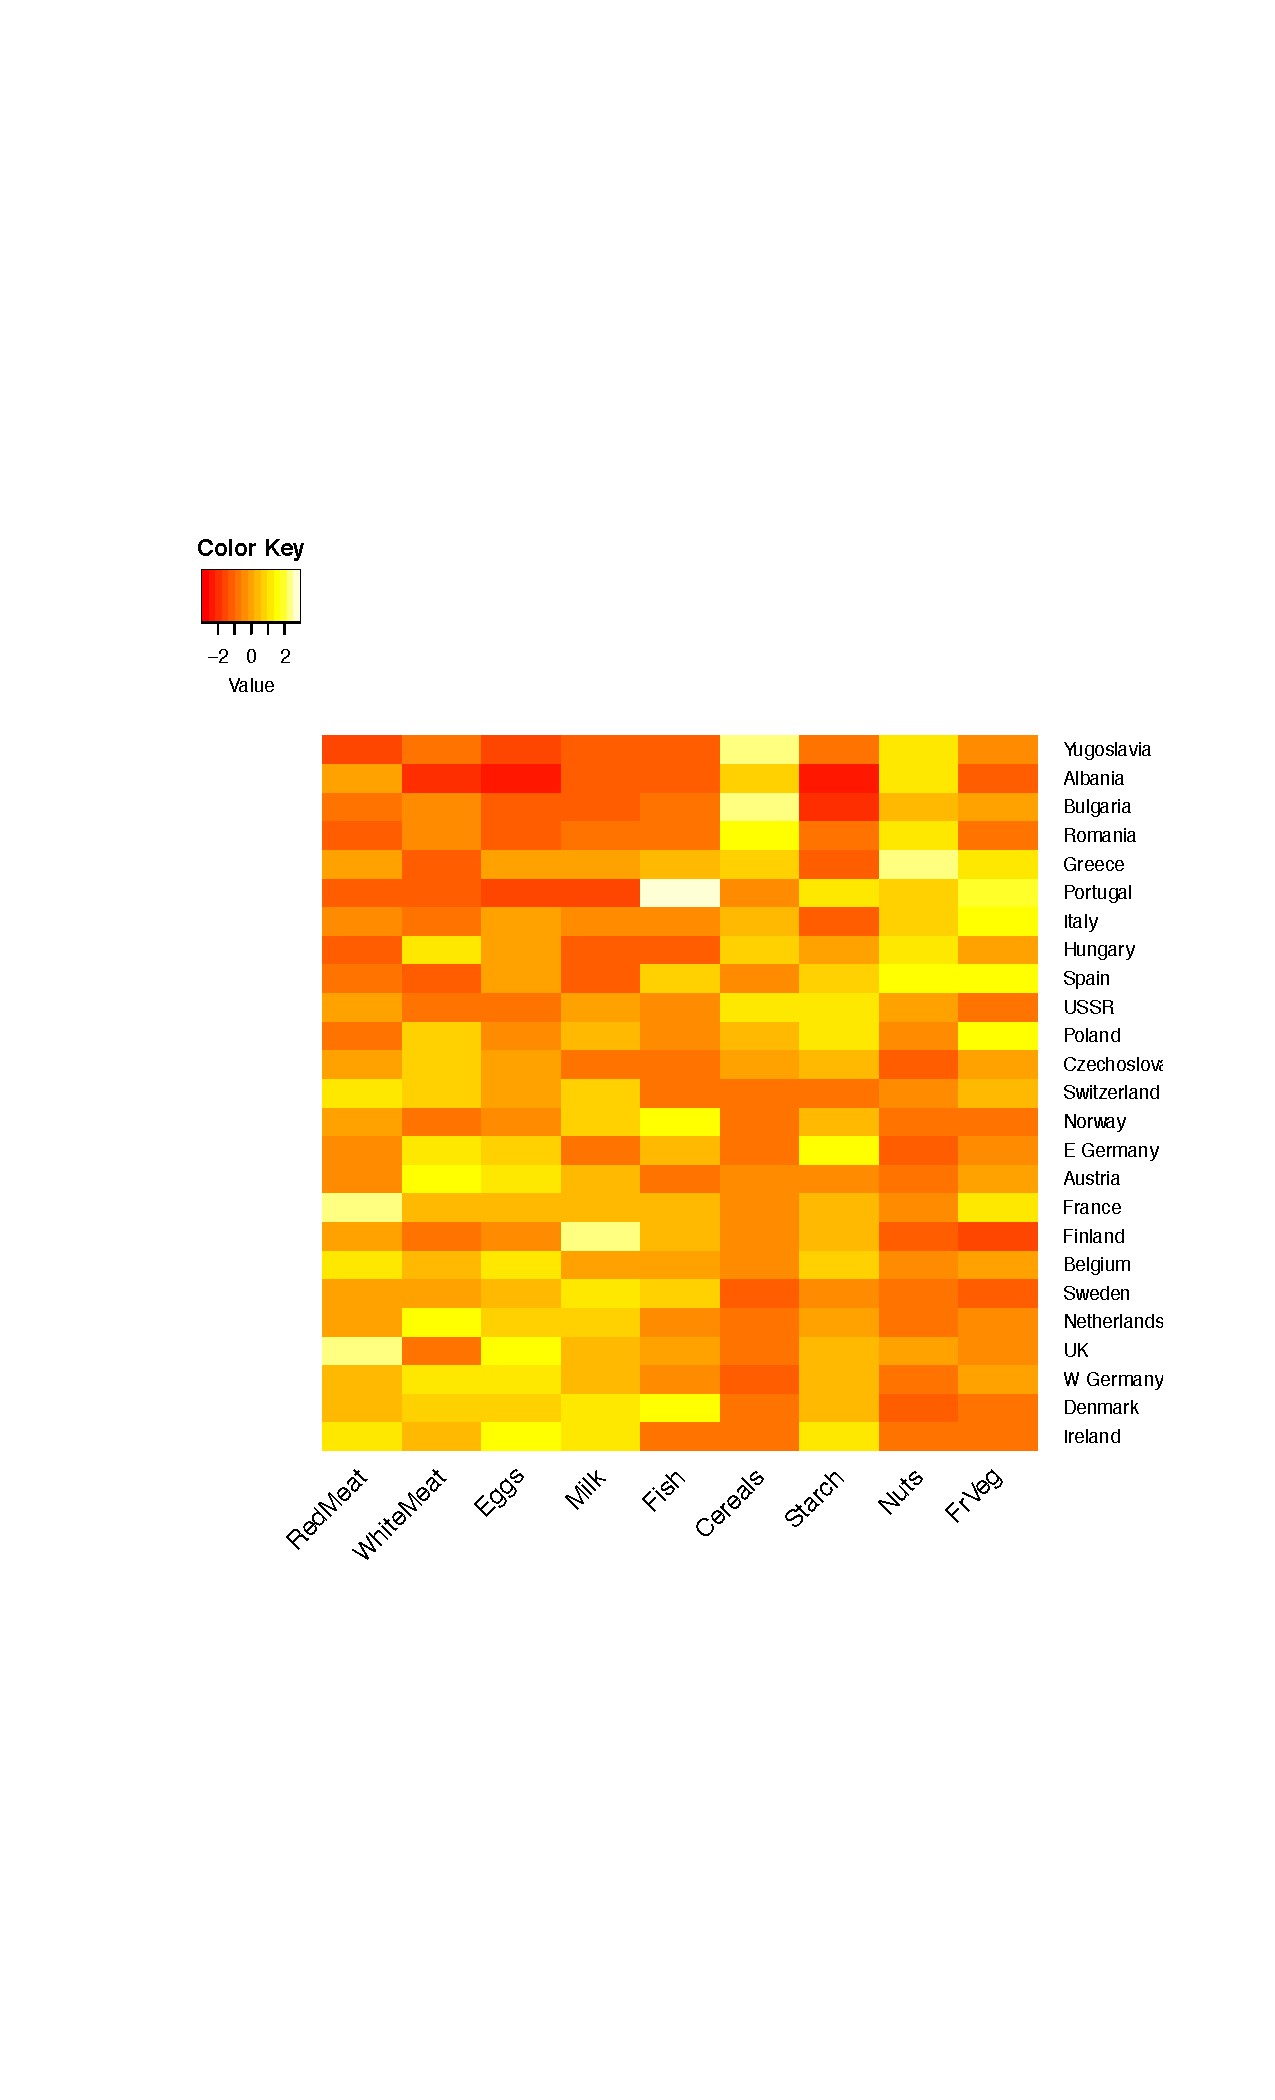
\includegraphics[width=\textwidth]{heatmap_pca.pdf}
    \caption{PCA}
    \label{fig:heat_pca}
  \end{subfigure}
  \caption{Heatmap, consumption of different products in different countries of Europe (quantitative measure of the amount of protein consumed). Anti-Robinson unweighted and PCA seriation, rescaled variables. \textit{Source: protein.txt}}
  \label{fig:heat_seriation}
\end{figure}


%---------------------------------- 
% Assignment 2

\section*{Assignment 2}

\subsection*{Wordcloud \& Phrase Net}


\begin{figure}[H]
  \begin{subfigure}[h]{0.5\textwidth}
    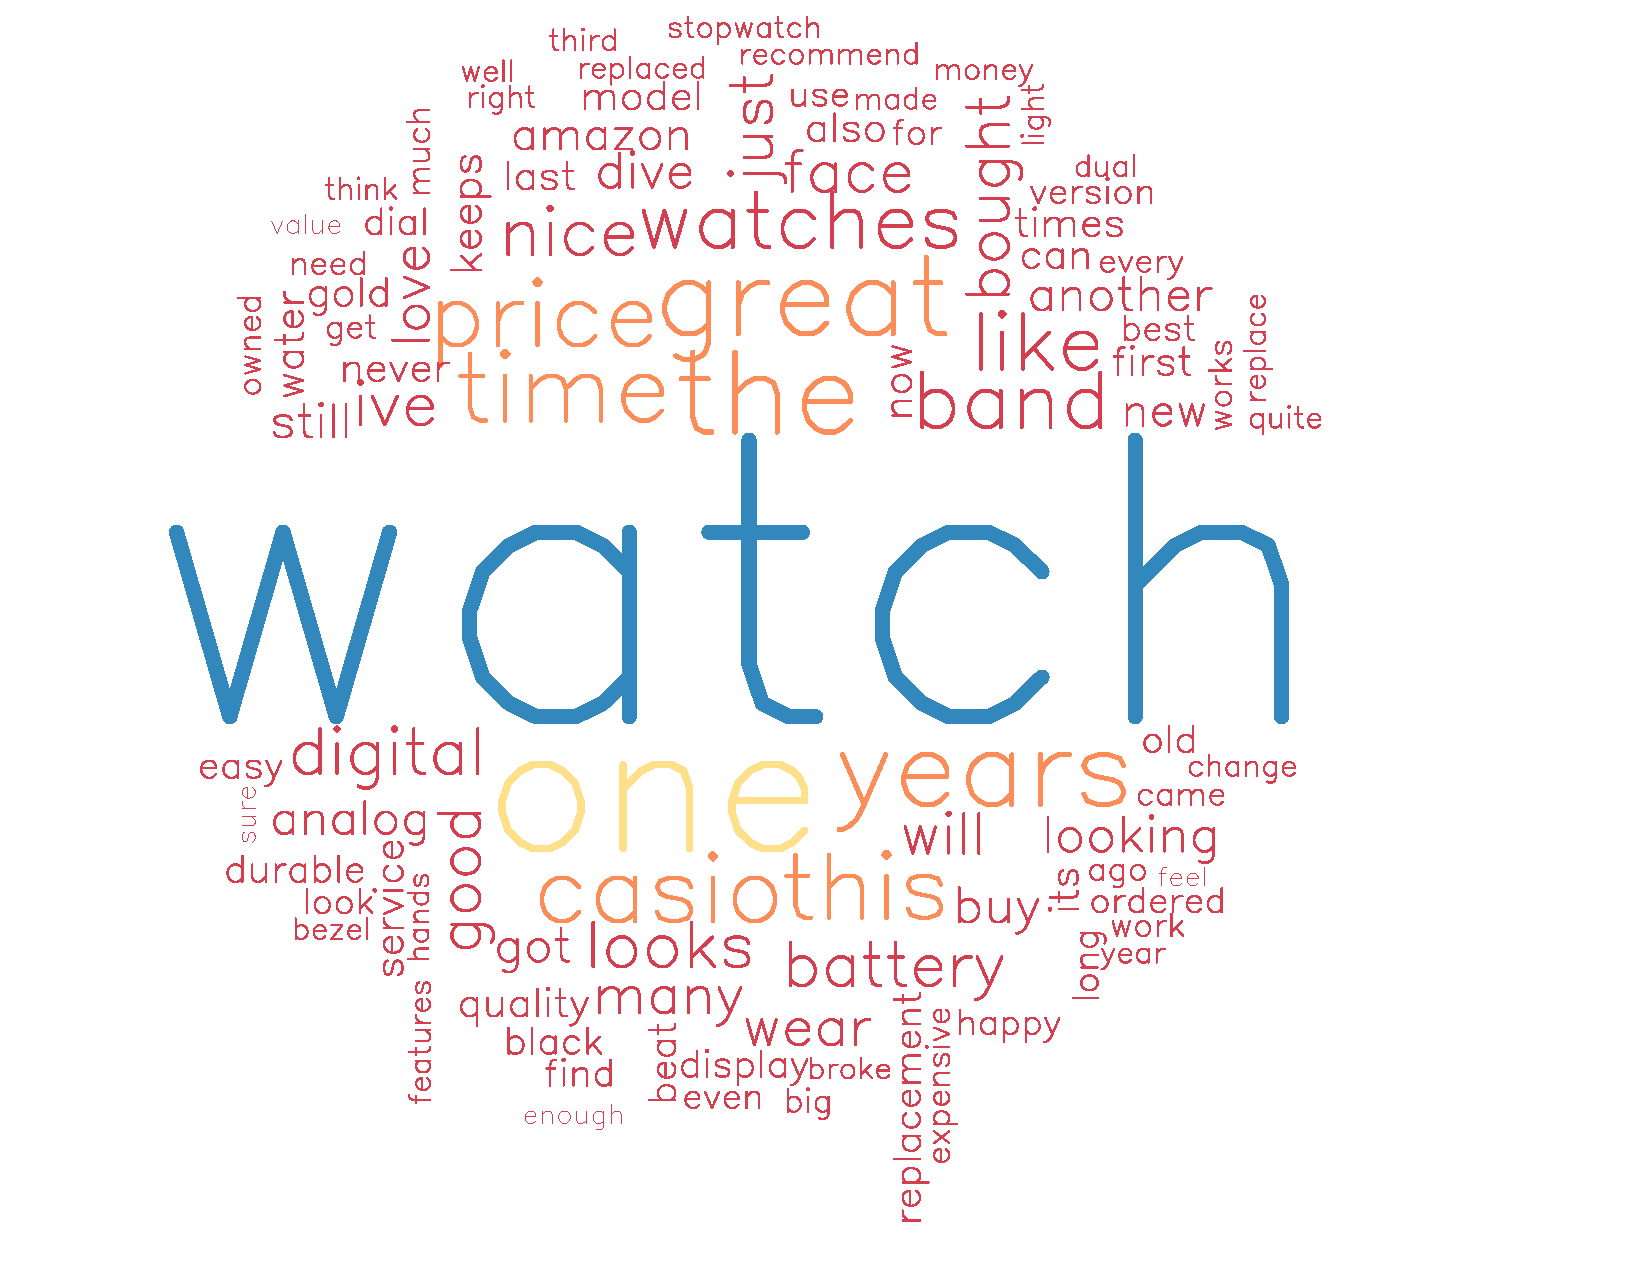
\includegraphics[width=\textwidth]{fivedata_wordcloud_mod.pdf}
    \caption{Satisfied costumers}
    \label{fig:five}
  \end{subfigure}
  %
  \begin{subfigure}[h]{0.5\textwidth}
    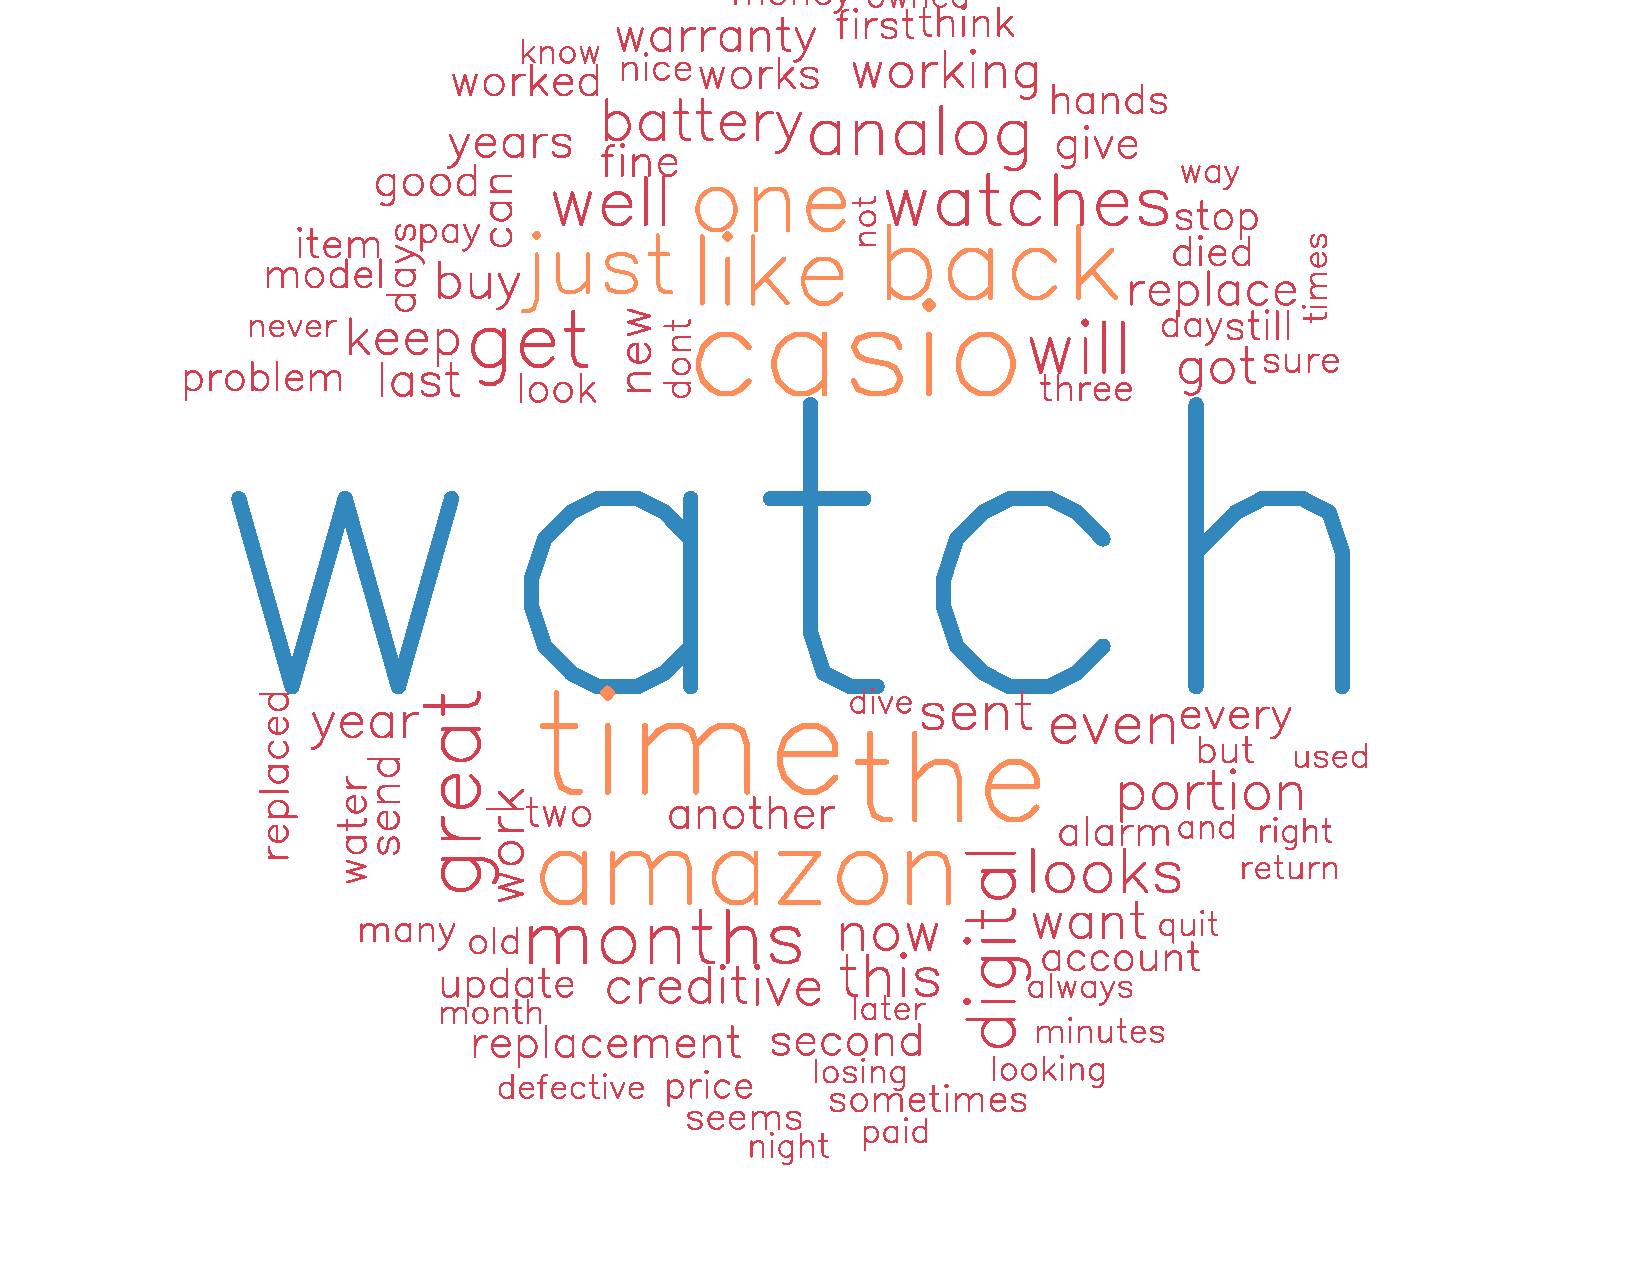
\includegraphics[width=\textwidth]{onetwo_wordcloud_mod.pdf}
    \caption{Not satisfied costumers}
    \label{fig:one_two}
  \end{subfigure}
  \caption{Wordcloud, feedbacks given by customers for watches Casio AMW320R-1EV bought at www.amazon.com. \textit{Source: Five.txt and OneTwo.txt}}
\end{figure}


%------------------------------------------------------
% Appendix

\lstset{
  frame=single,
  basicstyle=\ttfamily\footnotesize,
  commentstyle=\color{gray},
  frame=L,
  language=R,
  showstringspaces=false,
}


\newpage

\section*{Appendix}

\subsection*{R-Code}



\end{document}
